\chapter{드지터 지평선과 우주론적 확률}

\lectureoverview{지평선은 단순한 인과적 경계가 아니다. 정지 관측자에게 지평선은 열적 계다. 지평선에서 고유거리 \(\rho\)만큼 떨어진 곳에 둔 온도계는 대략 \(1/(2\pi\rho)\)의 온도를 가리키지만, 중력 적색편이 때문에 멀리서 관측되는 복사는 훨씬 더 차갑다. 블랙홀에서 얻은 이 교훈을 드지터 공간에 적용해 고정된 지평선 반지름 \(H^{-1}\)을 유도하고 관측자의 정적 패치 계량을 써 보겠다. 강의 후반부에서는 열역학이 이끄는 불편한 결과들, 즉 유한한 드지터 엔트로피, 푸앵카레 재귀, 볼츠만 브레인, 영원한 급팽창, 측도 문제를 살펴본다. 마지막으로 끈 이론의 정확한 초대칭 구조와 우리 우주를 기술할지도 모르지만 아직 알려지지 않은 틀을 구분해 논의한다.}

\section{지평선이 뜨겁다는 말의 의미}

강의를 본격적으로 시작하기 전에, 오늘 저녁의 논의 방향을 정하는 질문부터 살펴보자.

\begin{classroomqa}
\audiencequestion{우주 지평선에는 블랙홀이 없다. 그런데도 어떤 메커니즘으로 뜨거워질 수 있을까?\lecturetimestamp{00:00:17}}
\lecturerresponse{메커니즘은 블랙홀 지평선의 경우와 같다. 유용한 질문은 조작적이다. 지평선 가까이에 둔 온도계는 무엇을 기록하며, 지평선에서 멀리 떨어진 관측자에게는 어떤 복사가 도달하는가?}
\end{classroomqa}

첫 번째 실험은 국소적이다. 매끄럽고 비극한인 지평선에서 고유거리 \(\rho\)만큼 떨어진 곳에 온도계를 고정해 둔다. 지평선에 충분히 가까우면 기하학은 보편적인 린들러 형태를 띠며, 온도계는 다음 온도를 가리킨다.
\begin{equation}
T_{\rm local}(\rho)\simeq \frac{1}{2\pi\rho}
\label{eq:l09-local-temperature}
\end{equation}
\(\hbar=c=k_B=1\) 단위계에서 그렇다. 상수를 복원하면 다음과 같다.
\begin{equation}
k_B T_{\rm local}(\rho)\simeq \frac{\hbar c}{2\pi\rho}.
\end{equation}
\(\rho\to0\)일 때 발산한다고 해서 자유 낙하 관측자가 보통의 물질로 된 용광로를 만난다는 뜻은 아니다. 이 온도는 지평선 바로 바깥에 정지한 채 남아 있으려면 점점 더 큰 가속을 해야 하는 관측자가 부여하는 값이다.

도입부의 대화에서는 쉽게 혼동되는 세 가지 개념, 즉 에너지, 온도, 엔트로피도 구분한다.

\begin{classroomqa}
\audiencequestion{광자를 블랙홀 안으로 보내면 엔트로피는 여전히 같은 값으로 측정될까요, 아니면 에너지만 달라질까요?\lecturetimestamp{00:01:22}}
\lecturerresponse{광자가 지평선 너머로 들어가 더는 접근할 수 없게 되면 정보가 추가로 가려진다. 여기서 사용하는 단순화된 비트 표현으로는 광자 하나가 비트 하나를 더 숨겨 엔트로피를 증가시킬 수 있다. 에너지, 온도, 엔트로피는 서로 관련되어 있지만 서로 바꾸어 쓸 수 있는 개념은 아니다.}
\end{classroomqa}

\editorialnote{실제 블랙홀의 엔트로피 변화는 열역학적으로 \(dS=dE/T_H\)에 따라 정해지며, 에너지와 무관하게 모든 광자가 언제나 비트 하나에 해당하는 것은 아니다. 비트 하나라는 설명은 이 강의에서 사용한 정보이론적 이상화다.}

지평선 근처 영역에서는 고주파 양자 요동이 끊임없이 방출되고 다시 흡수된다. 지평선은 정지 관측자에게 이 요동을 열복사로 보이게 한다. 하지만 여기서 곧바로 의문이 생긴다. 그 영역이 임의로 뜨겁다면, 멀리 있는 관측자는 왜 임의로 에너지가 큰 광자 때문에 눈이 멀지 않을까?

\section{적색편이와 호킹 온도}

보통의 뜨거운 벽은 멀리 떨어져 있어도 고주파 복사의 근원으로 남는다. 지평선의 복사는 중력 적색편이를 거슬러 올라와야 한다는 점에서 다르다. 광자의 속력은 여전히 \(c\)이지만, 감소하는 것은 에너지다.
\begin{equation}
E=\hbar\omega,
\qquad
\omega_{\rm received}<\omega_{\rm emitted}.
\end{equation}
강의에서 든 분필 조각의 비유는 여기까지만 유효하다. 던진 돌은 올라가면서 느려지지만, 광자는 빛의 속력으로 계속 이동하는 동안 진동수와 에너지가 감소한다.

슈바르츠실트 블랙홀에서 무한대에 있는 관측자가 측정하는 온도는 다음과 같다.
\begin{equation}
T_H=\frac{1}{8\pi M}
\label{eq:l09-hawking-natural}
\end{equation}
\(G_N=\hbar=c=k_B=1\) 단위계에서 그렇다. 보통의 단위로 쓰면 다음과 같다.
\begin{equation}
T_H=\frac{\hbar c^3}{8\pi G_N M k_B}.
\label{eq:l09-hawking-full}
\end{equation}

\begin{figure}[htbp]
\centering
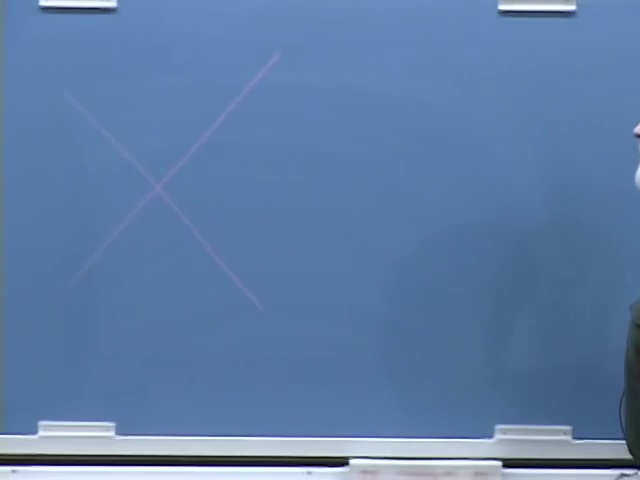
\includegraphics[width=0.68\textwidth]{lecture_09_figure_02.png}
\caption{자연 단위계에서의 호킹 온도 \(T_H=1/(8\pi M)\)}
\lectureframe{00:08:12}
\end{figure}

큰 블랙홀일수록 온도는 낮다. 강의에서는 대표적인 광자를 거슬러 추적해 이를 설명한다. 열복사의 광자는 특성 에너지 \(E_\gamma\sim T_H\)를 가진다. 무한대에 도달했을 때 에너지가 대략 \(M^{-1}\)인 광자는 지평선 가까이에서 출발할 때 훨씬 큰 국소 에너지를 지녔다. 지평선 근처 층에서 무한대까지의 적색편이는 블랙홀이 클수록 더 심해져, 점근 영역에서 측정되는 온도는 더 낮아진다.

\begin{classroomqa}
\audiencequestion{슈바르츠실트 시간이 지평선에서 멈춘다면, 처음에 안으로 떨어져 블랙홀을 만든 광자를 따라가야 할까요?\lecturetimestamp{00:04:19}}
\lecturerresponse{온도 문제를 살피려면 바깥쪽으로 방출된 광자를 따라가면 된다. 광자는 국소적으로 매우 높은 진동수에서 출발해 밖으로 올라오면서 에너지를 잃고 호킹 복사로 도달한다. 처음에 안으로 떨어진 광자의 운명은 별개의 정보 문제다.}
\end{classroomqa}

\section{플랑크 층과 늘어난 지평선}

식~\eqref{eq:l09-local-temperature}의 국소 관계는 어디까지 신뢰할 수 있을까? 강의에서는 반고전적 기술에서 플랑크 길이를 의미를 부여할 수 있는 최단 거리로 본다. 그러면 수학적 지평선에서 바깥쪽으로 대략 플랑크 길이만큼 떨어진 얇은 층에 플랑크 규모의 요동이 차 있는 그림이 떠오른다. 이 층에서는 방출과 흡수가 끊임없이 일어난다.

방출된 양자 가운데 대부분은 탈출하지 못한다. 아주 좁은 바깥쪽 원뿔 방향으로 나아가는 양자만 다시 떨어지지 않는다. 일반적인 각도로 방출된 양자는 지평선으로 되돌아온다. 바깥쪽으로 나가는 들뜸과 안쪽으로 들어오는 들뜸이 충돌해 쌍입자와 다른 입자들을 만들어 낸다. 이런 의미에서 정지 기술에는 극도로 뜨거운 물질로 된 얇은 껍질이 들어 있다.

\begin{figure}[htbp]
\centering
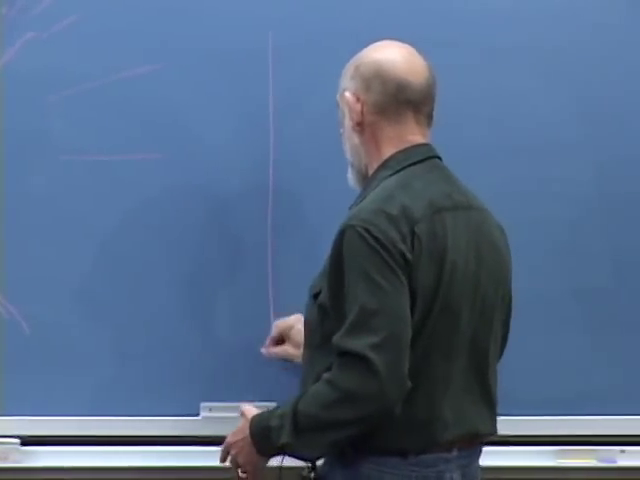
\includegraphics[width=0.74\textwidth]{lecture_09_figure_03.png}
\caption{지평선 근처 복사가 탈출할 수 있는 좁은 원뿔. 국소적으로 방출된 양자의 대부분은 지평선으로 되돌아온다.}
\lectureframe{00:11:38}
\end{figure}

이에 대응하는 시공간 그림도 있다. 지평선에서 멀리 떨어진 곳에서는 가상 요동을 짧은 닫힌 고리로 개략적으로 나타낼 수 있다. 입자와 반입자의 들뜸이 나타났다가 점근 상태가 되기 전에 사라진다는 뜻이다. 지평선 근처에서는 요동이 인과적 경계를 가로지를 수 있다. 외부 관측자에게는 바깥쪽 부분이 지평선에서 방출되었다가 나중에 다시 흡수되는 입자처럼 보인다. 그중 아주 작은 일부가 탈출해 호킹 복사가 된다.

\begin{classroomqa}
\audiencequestion{외부 영역의 그림에서 이런 요동은 \(t=-\infty\)에서 \(t=+\infty\)까지 이어지나요?\lecturetimestamp{00:15:00}}
\lecturerresponse{정확한 고전적 지평선을 사용하면 그런 특이해 보이는 기술이 나온다. 실제로는 지평선에서 플랑크 길이 정도 바깥에 있는 시간꼴 곡면인 늘어난 지평선으로 바꾸어 기술한다. 그러면 방출과 재흡수는 유한한 외부 시간에 일어난다.}
\end{classroomqa}

\begin{figure}[htbp]
\centering
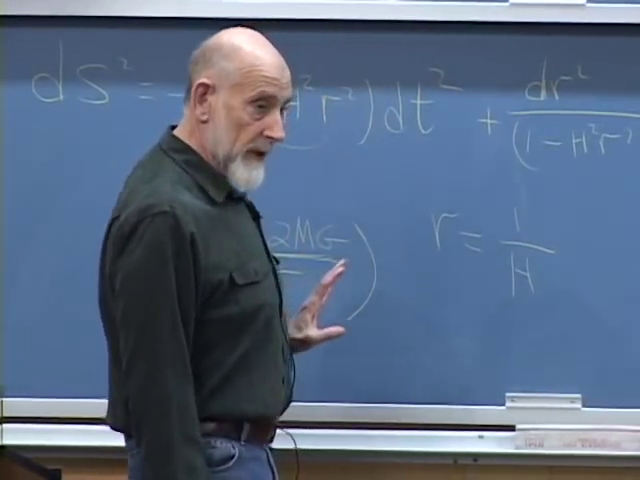
\includegraphics[width=0.72\textwidth]{lecture_09_figure_04.png}
\caption{외부 기술에서 사용하는 고전적 지평선과 그 가까이에 놓인 늘어난 지평선.}
\lectureframe{00:15:52}
\end{figure}

늘어난 지평선은 새로운 불변 경계가 아니다. 반고전적 기하학을 더는 신뢰할 수 없는 위치에 놓은 유효 곡면이다. 물질과 기하학 자체의 양자 요동은 지평선의 정확한 위치를 플랑크 규모로 흐릿하게 만든다. 이 구성에서는 그 불확실성을 하나의 곡면으로 나타내며, 그 위에서는 외부 기술이 유한한 값을 유지한다.

이 국소적 논의만으로는 지평선이 블랙홀에 속하는지 가속하는 우주에 속하는지 알 수 없다. 여기서 드지터 공간으로 넘어간다.

\section{팽창 좌표에서의 드지터 공간}

본 강의는 드지터 시공간의 공간적으로 평탄한 엽절단에서 시작한다.
\begin{equation}
ds^2=-dt^2+e^{2Ht}d\mathbf{x}^2,
\qquad
d\mathbf{x}^2=dx^2+dy^2+dz^2.
\label{eq:l09-flat-slicing}
\end{equation}
상수 \(H\)는 드지터 팽창률이다. 계량은 거리의 제곱을 재므로 인자는 \(e^{2Ht}\)로 나타난다. 좌표 간격이 고정되어 있을 때 물리적 길이는 다음과 같다.
\begin{equation}
D(t)=e^{Ht}\lvert\Delta\mathbf{x}\rvert.
\end{equation}

\begin{figure}[htbp]
\centering
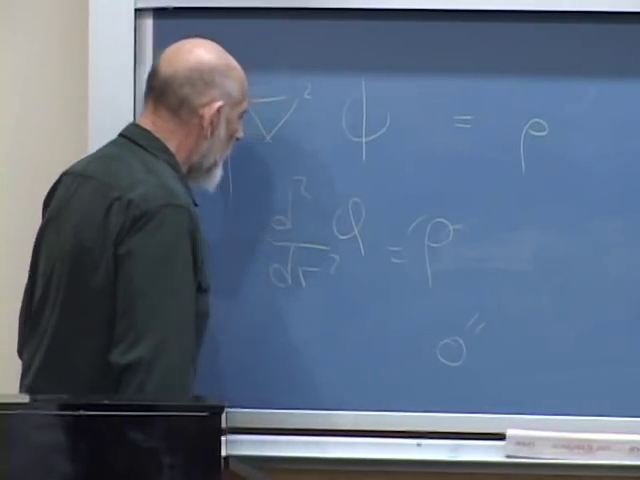
\includegraphics[width=0.78\textwidth]{lecture_09_figure_05.png}
\caption{평탄 좌표로 쓴 지수 팽창 드지터 계량.}
\lectureframe{00:18:50}
\end{figure}

이 좌표에서는 팽창이 명확히 드러나지만, 미래 무한대는 그림 위쪽으로 무한히 멀리 놓인다. 이를 칠판 안으로 가져오려면 등각 시간을 도입한다.
\begin{equation}
\eta=-\frac{1}{H}e^{-Ht},
\qquad
-\infty<\eta<0.
\label{eq:l09-conformal-time}
\end{equation}
그러면
\begin{equation}
dt=\frac{d\eta}{-H\eta},
\qquad
e^{Ht}=-\frac{1}{H\eta},
\end{equation}
이 되고, 식~\eqref{eq:l09-flat-slicing}은 다음과 같이 된다.
\begin{equation}
ds^2=\frac{1}{H^2\eta^2}
\left(-d\eta^2+d\mathbf{x}^2\right).
\label{eq:l09-conformal-metric}
\end{equation}
\(t\to+\infty\)일 때 \(\eta\to0^{-}\)이다. 무한한 고유시간이 유한한 수평선 \(\eta=0\)으로 압축되었다.

\editorialnote{칠판에 적는 동안 시간 변환식을 여러 번 고쳐 쓴다. 일관된 형태는 식~\eqref{eq:l09-conformal-time}이며, 초기 우주 시간은 \(\eta\to-\infty\)에 대응하고 미래 무한대는 \(\eta\to0^{-}\)에 대응한다.}

\begin{figure}[htbp]
\centering
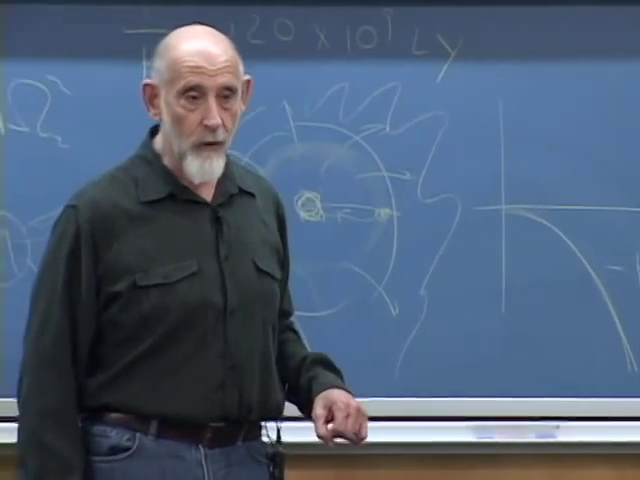
\includegraphics[width=0.82\textwidth]{lecture_09_figure_06.png}
\caption{등각 시간 변환과 등각 평탄 계량.}
\lectureframe{00:21:24}
\end{figure}

등각 인자는 시간 성분과 공간 성분 모두에 곱해지므로 영방향은 바뀌지 않는다. 방사형 광선에 대해서는
\begin{equation}
ds^2=0
\quad\Longrightarrow\quad
-d\eta^2+dx^2=0
\quad\Longrightarrow\quad
\frac{dx}{d\eta}=\pm1.
\label{eq:l09-null-rays}
\end{equation}
따라서 등각 도표에서 빛은 \(45^\circ\) 방향으로 이동한다. 좌표 변환이 유용한 이유가 여기에 있다. 인과적으로 도달할 수 있는 영역을 눈으로 확인할 수 있다.

\section{한 관측자의 인과 패치}

고유시간이 무한히 이어지는 관측자를 생각해 보자. 압축 도표에서 관측자의 세계선은 \(\eta=0\) 위의 한 점에서 끝난다. 관측자가 받을 수 있는 모든 신호는 그 끝점의 과거 광원뿔 안에 놓인다. 광원뿔 바깥의 사건은 관측자가 아무리 오래 기다려도 관측자와 정보를 주고받을 수 없다.

\begin{figure}[htbp]
\centering
\includegraphics[width=0.78\textwidth]{lecture_09_figure_07.png}
\caption{등각 드지터 좌표에서 관측자의 극한 과거 광원뿔.}
\lectureframe{00:24:38}
\end{figure}

다른 관측자에게는 다른 광원뿔이 있다. 두 관측자가 접근할 수 있는 영역은 겹치지만, 어느 쪽도 시공간 전체가 아니다. 이제부터는 첫 번째 관측자의 관점을 택하고, 그 과거 광원뿔을 관측자의 인과 패치라고 부르겠다.

그림만 보면 패치가 미래로 갈수록 줄어드는 듯하지만, 좌표상 폭은 고유거리가 아니다. 일정한 \(\eta\) 단면에서 관측자 \(x=0\)와 지평선 \(x=\Delta x\) 사이의 물리적 거리 제곱은 다음과 같다.
\begin{equation}
D^2=\frac{(\Delta x)^2}{H^2\eta^2}.
\label{eq:l09-horizon-distance-start}
\end{equation}
지평선은 \(45^\circ\) 영선이며 \(\eta=0\)에서 끝나므로
\begin{equation}
\Delta x=\lvert\eta\rvert.
\end{equation}
이를 대입하면
\begin{equation}
D_{\rm hor}^2=\frac{1}{H^2},
\qquad
D_{\rm hor}=\frac{1}{H}.
\label{eq:l09-horizon-radius}
\end{equation}
좌표상 간격은 줄어들지만 등각 인자는 그 감소를 정확히 상쇄할 만큼 커진다. 고유 지평선 반지름은 일정하다.

\begin{figure}[htbp]
\centering
\includegraphics[width=0.80\textwidth]{lecture_09_figure_08.png}
\caption{줄어드는 좌표 간격을 고정된 고유거리 \(H^{-1}\)로 바꾸는 칠판 유도.}
\lectureframe{00:28:42}
\end{figure}

\section{정적 패치}

고정된 지평선 반지름을 보면 중심 관측자에 맞춘 좌표를 도입할 수 있다. 좌표 변환을 유도하지 않고 강의에서는 결과를 바로 쓴다.
\begin{equation}
ds^2=
-\left(1-H^2r^2\right)d\tau^2
+\frac{dr^2}{1-H^2r^2}
+r^2d\Omega_2^2.
\label{eq:l09-static-patch}
\end{equation}
계수는 \(r\)에 의존하며 \(\tau\)에는 의존하지 않는다. 이 좌표계는 다음 범위의 관측자 정적 패치를 덮는다.
\begin{equation}
0\le r<\frac{1}{H}.
\end{equation}

\begin{figure}[htbp]
\centering
\includegraphics[width=0.88\textwidth]{lecture_09_figure_09.png}
\caption{드지터 정적 패치 계량과 슈바르츠실트 인자와의 비교.}
\lectureframe{00:34:22}
\end{figure}

슈바르츠실트 계량과의 유사성은 바로 드러난다.
\begin{equation}
f_{\rm dS}(r)=1-H^2r^2,
\qquad
f_{\rm Schw}(r)=1-\frac{2G_NM}{r}.
\end{equation}
두 경우 모두 정적 좌표에서 지평선은 \(f(r)=0\)인 곳에 생긴다. 드지터 공간에서는
\begin{equation}
1-H^2r^2=0
\quad\Longrightarrow\quad
r_H=H^{-1}.
\end{equation}
그곳에서 좌표계가 특이해지는데, 슈바르츠실트 좌표가 블랙홀 지평선에서 특이해지는 것과 같다. 그러나 전역적인 기하학은 중요한 점에서 다르다. 블랙홀 관측자는 바깥에 서서 안을 바라보지만, 드지터 관측자는 안에 서서 바깥을 바라본다.

\begin{classroomqa}
\audiencequestion{자유롭게 놓아둔 입자들이 지수적으로 팽창하는 우주에서 서로 멀어지는데, 기하학은 어떻게 정적일 수 있나요?\lecturetimestamp{00:36:06}}
\lecturerresponse{정적이라는 말은 모든 입자가 고정된 채 있다는 뜻이 아니다. 계량 계수와 반복 실험의 결과가 시작 시각에 의존하지 않는다는 뜻이다. 입자 두 개를 지금 놓아두면 서로 가속하며 멀어지고, 나중에 같은 실험을 반복해도 똑같은 운동이 일어난다.}
\end{classroomqa}

\begin{classroomqa}
\audiencequestion{서로 멀어지는 두 입자는 상대방의 빛이 적색편이되는 것을 보나요?\lecturetimestamp{00:38:34}}
\lecturerresponse{그렇다. 두 입자 사이의 거리가 늘어나므로 상대적 적색편이가 생긴다. 관측자에 맞춘 계량이 시간에 무관하더라도 그렇다.}
\end{classroomqa}

\section{내부에서 관측되는 온도}

슈바르츠실트 공간과 드지터 공간의 지평선 근처 구조는 국소적으로 동등하다. 따라서 드지터 지평선도 열적 양자를 방출하고 다시 흡수한다. 드물게 방출된 광자는 중심 관측자 쪽으로 안쪽을 향해 이동하면서 정적 패치의 중력 퍼텐셜을 거슬러 올라갈 때 에너지를 잃는다. 중심에서 측정되는 긴스버그--호킹 온도는 자연 단위계에서 다음과 같다.
\begin{equation}
T_{\rm dS}=\frac{H}{2\pi}
\label{eq:l09-de-sitter-temperature}
\end{equation}
반지름 \(r\)에 정지한 온도계는 톨먼 적색편이를 반영한 다음 온도를 읽는다.
\begin{equation}
T_{\rm local}(r)=
\frac{T_{\rm dS}}{\sqrt{1-H^2r^2}},
\label{eq:l09-tolman}
\end{equation}
이는 \(r\to H^{-1}\)일 때 발산하며, 지평선 근처에서는 식~\eqref{eq:l09-local-temperature}으로 돌아간다.

\editorialnote{강의에서는 식~\eqref{eq:l09-de-sitter-temperature}과 \eqref{eq:l09-tolman}을 명시적으로 쓰지 않고 지평선 거리와 적색편이로부터 온도 규모를 구한다. 이 식들은 그 논증의 표준적인 정규화를 나타낸다.}

현재 관측되는 후기 우주의 가속을 설명하기 위해 강의에서는 다음 주기 추정값을 사용한다.
\begin{equation}
H^{-1}\sim 20\times10^9\ {\rm light\ years}.
\label{eq:l09-lecture-horizon-estimate}
\end{equation}
그러면 전형적인 지평선 광자의 파장은 수십억 광년과 비슷한 규모가 된다. 이는 우주 마이크로파 배경 복사가 아니라, 그보다 훨씬 더 차가운 복사다.

조작적 사고실험은 우주론적 규모의 낚싯대와 같다. 앨리스는 \(r=0\)에 머물면서 데이터를 전송할 수 있는 매우 긴 줄에 온도계를 달고, 우주의 척력이 기기를 바깥으로 끌고 가게 둔다. 지평선 바로 앞에서 기기를 멈춘 뒤 신호가 돌아오기를 기다려 국소 온도가 높다는 것을 확인한다. 중심에 놓인 앨리스 곁의 온도계는 작은 값 \(H/(2\pi)\)을 가리킨다. 서로 다른 중력 퍼텐셜에서 측정했기 때문에 하나의 지평선에서 두 값이 모두 나타난다.

\section{지평선 통과}

고전적인 외부 관측 기술은 익숙한 블랙홀 이야기와 비슷하다. 중심에 있는 밥은 앨리스가 멀어지는 모습을 지켜본다. 앨리스의 신호는 점점 더 적색편이되고 도달 간격도 점점 길어진다. 앨리스는 지평선에 납작하게 달라붙은 듯 보이다가 결국 희미해진다. 나중에 여행을 떠난 제인은 경계 근처에 퇴적층처럼 쌓이는 또 하나의 더 얇은 층으로 보인다.

\begin{classroomqa}
\audiencequestion{우리의 관점에서 보면 물체는 우주 지평선을 실제로 통과하나요?\lecturetimestamp{00:45:30}}
\lecturerresponse{정적 관측자의 고전적 기술에서는 그렇지 않다. 물체의 겉보기 위치가 지평선에 다가가는 동안 신호는 적색편이되고 희미해진다. 그러나 물체와 함께 자유 낙하하는 관측자의 기술에서는 국소적으로 특이한 표면을 만나지 않고 지평선을 통과한다.}
\end{classroomqa}

\begin{classroomqa}
\audiencequestion{지평선은 통과하지 않은 채 가까이에 머무는 관측자에게만 뜨거운 건가요? 낙하 관측자는 지평선을 통과한다고 해서 타지는 않는 거죠?\lecturetimestamp{00:48:27}}
\lecturerresponse{앨리스는 자신의 기준계에서 지평선을 매끄럽게 통과한다. 극단적인 온도는 정지 관측자의 기술에서 나타난다. 밥이 지평선에 가까워지는 앨리스를 점점 더 자세히 관측하려면 점점 더 짧은 파장의 빛을 비춰야 한다. 하이젠베르크 현미경을 이용해 그렇게 관측하려 하면, 관측 대상이 탈 만큼의 에너지가 전달된다.}
\end{classroomqa}

이는 두 국소 사건 사이의 모순이 아니다. 정지 관측자와 낙하 관측자는 근본적으로 다른 측정을 한다. 지평선 상보성은 한 관측자가 중복된 정보를 직접 대조할 수 없으면서도 두 기술이 모두 타당할 수 있는 방법을 묻는다.

\section{진공 척력을 설명하는 뉴턴 모형}

이때 한 학생이 블랙홀의 중력 우물에 해당하는 것이 무엇인지 묻는다. 서스킨드는 뉴턴 모형을 구성해 답한다. 중력 퍼텐셜을 \(\phi\)라 하면 시험 입자의 가속도는 다음과 같다.
\begin{equation}
\mathbf{a}=-\boldsymbol{\nabla}\phi.
\end{equation}
보통의 비상대론적 물질에 대해서는 푸아송 방정식이 다음과 같다.
\begin{equation}
\nabla^2\phi=4\pi G_N\rho.
\label{eq:l09-poisson}
\end{equation}

\begin{classroomqa}
\audiencequestion{블랙홀 효과가 중력 우물에서 생긴다면, 드지터 공간에서는 무엇이 이에 대응하는 원천인가요?\lecturetimestamp{00:49:36}}
\lecturerresponse{진공 에너지 자체가 공간적으로 균일한 중력 원천을 제공한다. 뉴턴 기술에서는 이것이 \(1/r\) 우물이 아니라 이차 퍼텐셜을 만든다.}
\end{classroomqa}

\begin{figure}[htbp]
\centering
\includegraphics[width=0.78\textwidth]{lecture_09_figure_10.png}
\caption{푸아송 방정식과 강의에서 개략적으로 쓴 방사형 이계도함수 형태.}
\lectureframe{00:51:38}
\end{figure}

칠판의 유도에서는 정규화와 구면 좌표의 측도 항, 압력을 생략하고 처음에는 전체 부호까지도 생략해 문제를 다음과 같이 단순화한다.
\begin{equation}
\frac{d^2\phi}{dr^2}\sim H^2.
\end{equation}
핵심적인 추론은 원천이 일정하면 이차함수가 된다는 것이다. 드지터 척력에 맞는 부호를 택하면
\begin{equation}
\phi_{\rm dS}(r)=-\frac{1}{2}H^2r^2,
\qquad
a_r=-\frac{d\phi_{\rm dS}}{dr}=H^2r.
\label{eq:l09-de-sitter-potential}
\end{equation}
가속도는 바깥쪽을 향하며 거리에 비례해 커진다. \(\ddot r=H^2r\)을 풀면
\begin{equation}
r(\tau)=A e^{H\tau}+B e^{-H\tau},
\end{equation}
을 얻으므로, 증가하는 해가 지수적 분리를 재현한다.

\begin{figure}[htbp]
\centering
\includegraphics[width=0.76\textwidth]{lecture_09_figure_11.png}
\caption{균일한 원천을 나타내는 방정식과 드지터 이차 퍼텐셜.}
\lectureframe{00:53:32}
\end{figure}

\editorialnote{일반 상대론에서 균일한 유체의 약한 장 근사 가속도는 \(\rho+3p\)에 의존하며 \(\rho\)에만 의존하지 않는다. 진공 에너지는 \(p=-\rho\)이므로 \(\rho+3p=-2\rho\)이고, 이에 따라 가속도는 척력으로 작용한다. 식~\eqref{eq:l09-de-sitter-potential}은 정규화를 올바르게 적용한 드지터 결과다. 칠판의 계산에서는 이차 의존성과 부호만 살펴본다.}

중심에 보통의 질량 \(M\)를 놓아 보자. 그러면 퍼텐셜은 정성적으로 다음과 같이 된다.
\begin{equation}
\phi(r)=-\frac{G_NM}{r}-\frac{1}{2}H^2r^2,
\label{eq:l09-combined-potential}
\end{equation}
방사 방향 가속도는
\begin{equation}
a_r=-\frac{G_NM}{r^2}+H^2r.
\end{equation}
이다. 작은 \(r\)에서는 국소적인 인력이 우세하고, 큰 \(r\)에서는 진공 척력이 우세하다. 두 효과가 균형을 이루는 위치는 다음과 같다.
\begin{equation}
r_\ast=\left(\frac{G_NM}{H^2}\right)^{1/3}.
\label{eq:l09-turnaround}
\end{equation}
이것이 강의에서 그린 퍼텐셜 최대점을 더 명확히 나타낸 결과다. 가까운 중력 결합계는 서로 붙어 있을 수 있지만 충분히 멀리 떨어진 은하들은 가속하며 멀어지는 이유를 정성적으로 설명해 준다.

\begin{figure}[htbp]
\centering
\includegraphics[width=0.78\textwidth]{lecture_09_figure_12.png}
\caption{보통의 \(1/r\) 인력과 위가 아래로 향한 포물선 모양의 드지터 퍼텐셜을 합친 결과.}
\lectureframe{00:58:20}
\end{figure}

\begin{classroomqa}
\audiencequestion{보통의 힘도 여전히 중요한가요, 아니면 진공 척력이 결국 모든 물질의 섬을 찢어 놓나요?\lecturetimestamp{00:57:29}}
\lecturerresponse{모든 힘을 고려해야 한다. 충분히 작은 규모에서는 전자기적 결합과 국소 중력이 우세하다. 진공 척력은 \(H^{-1}\)과 결합 질량에 맞는 균형 규모로 정해지는 엄청나게 큰 거리에 걸쳐서만 중요해진다.}
\end{classroomqa}

\section{하나의 원천, 여러 이름}

이제 논의는 용어를 짚어 보며 잠시 멈춘다. 여기서 사용하는 모형에서 진공 에너지, 우주 상수, 암흑 에너지는 서로 더해지는 세 가지 물질이 아니다. 이들은 같은 \(w=-1\) 원천을 세 가지 방식으로 기술한 것이다. 아인슈타인 방정식의 상수항, 진공의 로런츠 불변 에너지 밀도, 후기 우주 가속을 일으키는 성분이라고 부를 수 있다.

\begin{classroomqa}
\audiencequestion{균일한 뉴턴 원천과 양자 진공 에너지가 별개의 효과로 함께 존재하나요?\lecturetimestamp{00:59:14}}
\lecturerresponse{아니다. 균일한 밀도는 같은 원천을 뉴턴 모형으로 나타낸 것이다. 진공 에너지, 우주 상수, 그리고 이 강의에서 말하는 암흑 에너지는 하나의 물리적 성분을 가리킨다.}
\end{classroomqa}

\begin{classroomqa}
\audiencequestion{그렇다면 같은 현상을 고전적으로도, 양자역학적으로도 기술할 수 있나요?\lecturetimestamp{01:00:32}}
\lecturerresponse{전자 질량의 일부가 양자적 기원을 갖듯이, 그 미시적 기원은 양자역학적일 수 있다. 유효 에너지 밀도를 알게 되면 그것은 고전 중력 방정식에 보통의 원천으로 들어간다. 관측된 값의 궁극적인 기원은 아직 모른다.}
\end{classroomqa}

플랑크 단위계에서 관측된 진공 에너지 밀도는 엄청나게 작다.
\begin{equation}
\rho_\Lambda\sim10^{-123}\rho_{\rm Pl},
\label{eq:l09-planck-smallness}
\end{equation}
정확한 값은 플랑크 밀도에 사용하는 관례에 따라 달라진다. 이 작은 값이 우주 상수 문제다. 지평선이 그토록 큰 이유도 여기에 있다. 4차원에서는
\begin{equation}
H^2=\frac{8\pi G_N}{3}\rho_\Lambda,
\qquad
r_H=H^{-1}.
\end{equation}
\(H\)가 더 크다면 지평선은 더 작아지고 중심의 드지터 온도는 더 높아지며, 척력 가속도 \(H^2r\)도 더 강해질 것이다.

\begin{classroomqa}
\audiencequestion{작은 우주 상수는 플랑크 상수 및 양자 요동과 관련이 있나요?\lecturetimestamp{01:03:27}}
\lecturerresponse{깔끔하게 비교하려면 무차원 플랑크 단위계를 사용하면 된다. 이 단위계에서는 \(G_N=\hbar=c=1\)이다. 그 단위계에서 진공 밀도는 자연스러운 플랑크 밀도보다 약 \(123\) 자릿수만큼 작다. 이 계층을 설명하는 것은 기초 물리학의 핵심 난제 가운데 하나다.}
\end{classroomqa}

\begin{classroomqa}
\audiencequestion{진공 에너지는 반드시 정확히 일정한 우주 상수여야 하나요? 가속을 일으키는 성분이 줄어들다가 결국 0에 이를 수도 있나요?\lecturetimestamp{01:04:52}}
\lecturerresponse{논리적으로 가능한 대안이다. 동역학적 암흑 에너지 장은 시간에 따라 변할 수 있다. 강의에서 상수인 경우를 택한 것은 당시 이용 가능했던 관측이 우주 상수에 가까운 거동을 점점 더 지지했기 때문이지, 모든 대안이 불가능하다고 입증되었기 때문은 아니다.}
\end{classroomqa}

\section{먼 미래의 천문학}

점근적으로 드지터인 우주에서는 중력적으로 묶여 있지 않은 구조들이 결국 관측자의 지평선을 넘어간다. 우주 마이크로파 배경 복사는 검출할 수 없는 수준으로 적색편이된다. 먼 은하들은 시야에서 사라진다. 살아남은 천문학자는 어둠에 잠긴 패치 안에서 하나로 합쳐진 국소 중력 섬만 보게 될 수도 있다.

\begin{classroomqa}
\audiencequestion{망원경이 없다면 먼 은하들이 사라진 사실조차 알아차릴 수 있을까요?\lecturetimestamp{01:06:17}}
\lecturerresponse{아마 알아차리지 못할 것이다. 더 근본적인 문제는 이렇다. 미래 관측자들은 정교한 장비를 갖추더라도 오늘날 우리가 팽창을 추론하는 데 쓰는 먼 천체와 우주 마이크로파 배경을 잃어버릴 수 있다.}
\end{classroomqa}

그렇다면 오래된 섬 우주 모형이 설득력 있어 보일 수 있다. 올베르스의 역설도 다른 결론을 강요하지 않을 것이다. 올베르스의 역설은 광원을 내는 천체들이 무한하고 정적이며 균일하게 분포한다고 가정하지만, 미래 관측자가 보게 되는 것은 국소적인 섬 안에 있는 유한한 수의 별뿐이기 때문이다. 암흑 에너지가 빈 공간에서 대체 은하를 계속 만들어 내는 것은 아니다.

정확한 드지터 공간에서 지평선은 국소 은하를 중심으로 줄어들지 않는다. 물리적 반지름 \(H^{-1}\)은 은하보다 훨씬 크며 일정하게 유지된다. 사라지는 것은 고정된 인과적 경계 너머로 실려 가는 비결합 물질이다.

\begin{classroomqa}
\audiencequestion{은하에서 튕겨 나간 별들을 큰 규모의 기하학을 검출하기 위한 시험체로 쓸 수 있을까요?\lecturetimestamp{01:11:25}}
\lecturerresponse{한동안은 가능하다. 방출된 천체와 긴 기준선에 걸친 빛 신호로 기하학을 탐사할 수 있다. 하지만 효과가 뚜렷해지는 것은 십억 광년의 상당 부분에 해당하는 거리 규모에서뿐이므로, 실험에는 우주론적 시간이 걸릴 것이다.}
\end{classroomqa}

\begin{classroomqa}
\audiencequestion{먼 지평선이 이미 우주의 대부분을 우리에게서 가리고 있지는 않다는 것을 어떻게 알 수 있나요?\lecturetimestamp{01:11:45}}
\lecturerresponse{우리는 팽창을 측정하고 대규모 기하학을 재구성할 만큼 충분한 은하, 적색편이, 배경 복사를 이미 관측하고 있다. 그런 추적 수단을 잃게 될 미래 관측자에게는 추론이 훨씬 더 어려울 것이다.}
\end{classroomqa}

\begin{classroomqa}
\audiencequestion{지평선이 안드로메다 바로 너머에 있다면 그 존재가 분명히 드러날까요?\lecturetimestamp{01:12:19}}
\lecturerresponse{그렇다. 그렇게 작은 지평선이려면 \(H\)가 훨씬 더 커야 하고, 그에 따른 척력이 안드로메다의 운동을 크게 바꿀 것이다. 실제로 측정된 값에 따르면 점근적 지평선의 규모는 그보다 훨씬 크다.}
\end{classroomqa}

\begin{classroomqa}
\audiencequestion{우리 지평선 너머에서 새로운 빅뱅이 일어나고 있을 수도 있나요?\lecturetimestamp{01:13:25}}
\lecturerresponse{지평선 너머의 사건은 우리에게도 후손에게도 보이지 않는다. 이와 관련되면서 더 정확하게 말할 수 있는 가능성인 영원한 급팽창에서의 거품 핵생성은 강의 뒷부분에서 소개한다.}
\end{classroomqa}

로켓과 시계, 그리고 수십억 년의 시간이 있다면 미래 관측자들은 패치의 상당 부분을 가로질러 탐사선을 보내고 계량을 재구성할 수 있다. 그러나 보통의 실험실 시간이나 문명이 존속하는 시간 규모에서는 그 효과에 접근하기가 거의 불가능하다. 이 구분을 통해 팽창을 발견할 수 없다는 지나치게 강한 주장을 바로잡을 수 있다. 원리적으로 금지된 것이 아니라, 실제로 확인하기까지 우주론적 규모의 시간이 걸리는 것이다.

\begin{classroomqa}
\audiencequestion{미래의 탐사자들이 열적 재귀를 기다리는 것보다 훨씬 일찍 기하학을 알아낼 수 있나요?\lecturetimestamp{01:21:40}}
\lecturerresponse{물론이다. 재귀를 측정 방법으로 제안하는 것이 아니다. 십억 광년 규모의 기준선에 걸쳐 빛 신호를 주고받는 탐사자들은 훨씬 짧은 시간 안에 정적 패치를 지도화할 수 있다. 물론 그 시간도 우주론적 규모이기는 하다.}
\end{classroomqa}

\begin{classroomqa}
\audiencequestion{그런 탐사자들이 보내오는 정보가 적색편이 때문에 모두 사라질까?\lecturetimestamp{01:23:24}}
\lecturerresponse{그들이 지평선 안쪽의 충분히 작은 규모를 탐사한다면 그렇지 않다. 십억 광년 정도의 기준선만으로도 팽창에 민감해지면서 적색편이는 중간 정도에 그친다. 이 실험은 주로 엄청나게 긴 시간 때문에 제약을 받는다.}
\end{classroomqa}

\section{유한한 엔트로피와 재귀}

정적 패치는 열역학적 의미에서 비어 있지 않습니다. 그 지평선의 면적은
\begin{equation}
A_H=4\pi H^{-2},
\end{equation}
온도는 \(T_{\rm dS}=H/(2\pi)\)이며, 엔트로피는
\begin{equation}
S_{\rm dS}=\frac{A_H}{4G_N}
=\frac{\pi}{G_NH^2}
\label{eq:l09-de-sitter-entropy}
\end{equation}
단위계 \(\hbar=c=k_B=1\)에서 주어집니다. 엔트로피는 유한합니다. 따라서 적절한 주의를 기울인다면, 정적 패치를 정상적인 기술에서 들뜸이 지평선 부근에 집중된 유한 엔트로피 열적 공동으로 그려 볼 수 있습니다.

평형 상태의 보통 기체 상자는 짧은 시간 척도에서는 아무런 특징도 없어 보이지만, 통계역학은 요동을 금지하지 않습니다. 어떤 거시 상태의 엔트로피가 평형 상태보다 \(\Delta S\)만큼 낮다면, 그 상태의 확률은 대략
\begin{equation}
P\sim e^{-\Delta S}.
\label{eq:l09-fluctuation-probability}
\end{equation}
기다리는 시간은 이에 따라
\begin{equation}
t\sim t_0 e^{\Delta S}.
\end{equation}
만큼 늘어납니다. 유한한 계가 이전 상태와 임의로 가까운 상태를 다시 방문하기까지 걸리는 시간은 푸앵카레 재귀 시간이며,
\begin{equation}
t_{\rm rec}\sim H^{-1}e^{S_{\rm dS}}.
\label{eq:l09-recurrence}
\end{equation}
우리 지평선의 \(S_{\rm dS}\)가 대략 \(10^{120}\) 규모이므로, 강의에서는 그 척도를 \(e^{10^{120}}\)로 요약합니다. 앞의 계수가 연 단위인지, 허블 시간 단위인지, 미시적 단위인지는 이중 지수에 비하면 중요하지 않습니다.

\begin{figure}[htbp]
\centering
\includegraphics[width=0.76\textwidth]{lecture_09_figure_13.png}
\caption{칠판에 엄청난 지수적 대기 시간이 적힌 재귀 논의.}
\lectureframe{01:16:24}
\end{figure}

그러한 재귀가 일어나기 전에도 더 작은 요동은 훨씬 흔합니다. 방 안의 분자들이 모두 한쪽 구석에 모일 수도 있고, 복잡한 소용돌이가 잠시 생길 수도 있습니다. 강의에서 장난스럽게 나열한 예로는 열운동이 코끼리를 조립할 수도 있습니다. 필요한 엔트로피 감소가 작을수록 요동에 드는 비용도 낮습니다.

\begin{classroomqa}
\audiencequestion{푸앵카레 재귀는 양자역학의 고유한 결과인가요?\lecturetimestamp{01:25:44}}
\lecturerresponse{아닙니다. 재귀와 희귀한 요동은 고전 통계역학에서도 이미 나타납니다. 이를 드시터 공간에 적용하는 것은 언젠가 수정될 수도 있는 현재의 물리적 틀에 기반하지만, 열역학과 통계적 추론은 우리가 아는 가장 견고한 체계에 속합니다.}
\end{classroomqa}

확률 자체의 의미는 미래 이론에서 더 깊어질 수도 있습니다. 서스킨드는 그렇지 않다고 주장하지 않습니다. 그가 말하는 더 제한적인 요점은, 장시간에 걸친 함의가 낯설다는 이유만으로 통계역학을 버리면 물리학에서 가장 잘 검증된 구성 원리 중 하나를 포기하게 된다는 것입니다.

\section{볼츠만 두뇌와 전형적인 관측자}

열적 요동이 빅뱅과 비슷한 상태 전체를 만들어 낸다고 가정해 봅시다. 그러려면 엔트로피가 엄청나게 감소해야 합니다. 태양계 하나를 만들어 내는 요동은 비용이 더 적고, 이미 따뜻한 지구를 만들어 내는 요동은 그보다도 비용이 적습니다. 필요한 것이 관측자 하나뿐이라면, 가장 비용이 적은 요동은 겉보기 기억을 온전히 갖춘 기능하는 뇌만 만들어 낼 수도 있습니다. 이런 가상의 관측자를 볼츠만 두뇌라고 부릅니다.

쟁점은 기이한 요동 하나가 논리적으로 가능한지 여부가 아닙니다. 우주론 모형이 거의 모든 관측자를 그런 요동으로 만들어진 관측자라고 예측하는지가 문제입니다. 우리는 자신이 터무니없이 비전형적인 경우가 아니라고 가정하고 관측 결과를 추론합니다. 일관된 우주 역사를 지닌 보통의 관측자보다 고립된 열적 두뇌가 지수적으로 더 많다고 보는 이론은 그런 추론의 근거를 흔듭니다.

따라서 볼츠만 두뇌 문제는 정량적인 일관성 검사를 가리킵니다. 보통의 관측자가 얼마나 있을지와 요동으로 생겨난 관측자가 얼마나 있을지를 비교합니다. 후자가 우세하다면 진공이 그들이 증식하기 전에 붕괴해야 하거나, 측도를 바꾸거나, 우주론의 가정을 재검토해야 합니다.

자외선--적외선 연결에 관한 앞선 질문은 여기서 명시적으로 미뤄 둡니다. 재귀 논증은 그 별개의 문제를 해결하지 않아도 성립합니다.

\section{영원한 인플레이션과 거품 우주}

다음으로 강의는 완전한 유도를 시도하지 않은 채 두 번째 확률 문제를 소개합니다. 준안정 드시터 진공에서는 진공 에너지가 더 낮은 거품이 핵생성될 수 있습니다. 거품 벽은 팽창하고, 내부는 열린 프리드먼--로버트슨--워커 우주로 진화할 수 있습니다. 한편 주위의 인플레이션 영역은 계속 팽창하면서 거품을 더 만들어 냅니다.

\begin{figure}[htbp]
\centering
\includegraphics[width=0.74\textwidth]{lecture_09_figure_14.png}
\caption{인플레이션하는 드시터 배경 안에 그려진, 진공 에너지가 더 낮은 거품.}
\lectureframe{01:29:38}
\end{figure}

핵심은 개체 수가 지수적으로 늘어난다는 점입니다. 새로운 물리적 부피가 거품이 제거하는 부피보다 더 빠르게 생겨나므로, 거품 영역의 수는 한없이 증가합니다. 거품마다 서로 다른 낮은 에너지 상태에 자리 잡을 수 있으므로, 유효한 물리 법칙도 서로 다를 수 있습니다.

통계적 어려움을 드러내기 위해, Susskind는 먼저 우주론을 떠나 자원은 유한하지만 그 양은 알려지지 않은 상황에서 인구가 지수적으로 증가하는 경우를 생각한다. 살았거나 앞으로 살아갈 모든 사람 가운데 관측자가 전형적이라고 가정하자. 인구가 세대마다 두 배로 늘다가 어느 시점에 끝난다면, 전체 인구의 절반은 마지막 세대에 살고, 사분의 삼은 마지막 두 세대에, 팔분의 칠은 마지막 세 세대에 산다.
\begin{equation}
f_n=1-2^{-n}.
\label{eq:l09-last-generations}
\end{equation}
그렇다면 전형성에 따르면 우리는 불편할 만큼 종말에 가까운 시기에 살고 있는 셈이다. 총 자원 공급량에 대해 아무것도 모른다 해도 그렇다. 이는 인류 멸종을 신뢰할 만하게 예측하려는 주장이 아니다. 지수적 성장이 집계 결과를 절단값에 좌우되게 만든다는 경고다.

동전 던지기 예시는 보통의 전형성 가정을 더 명료하게 보여 줍니다. 많은 실험자가 각각 공정한 동전을 \(N\)번 던진다면, 압도적 다수는
\begin{equation}
n_H=\frac{N}{2}+O(\sqrt{N}).
\end{equation}
을 얻습니다. 극단적으로 드문 결과를 얻은 관측자라면, 근거도 없이 자신이 터무니없이 희귀한 꼬리 부분에 있다고 가정하기보다 먼저 모형이나 동전에 문제가 있는지 의심해야 합니다. 우주론에서 확률을 다룰 때도 같은 전형성 직관을 사용하지만, 모집단이 무한하다면 잘 정의된 계수 방법이 필요합니다.

\section{에셔의 경계와 측도 문제}

서스킨드가 든 기하학적 비유는 M.\ C.\ 에셔의 \emph{원형 극한 IV}입니다. 원반을 천사와 악마가 채우고 있으며, 경계에 가까워질수록 도형이 작아 보입니다. 이 그림이 나타내는 쌍곡기하학에서는 도형들이 서로 동등하며, 유클리드적으로 보이는 크기만 투영 때문에 달라집니다.

\begin{figure}[htbp]
\centering
\includegraphics[width=0.76\textwidth]{lecture_09_figure_15.png}
\caption{원형 경계 가까이에서 지수적으로 증식하는 도형을 대신해 칠판에 그린 그림.}
\lectureframe{01:37:54}
\end{figure}

에셔에게 주어진 시간과 잉크, 인내심이 유한하다고 상상해 봅시다. 그는 가장자리 가까이에서 결국 그리기를 멈추고, 몇몇 도형은 미완성으로 남겨 둘 수도 있습니다. 쌍곡 반지름에 따라 도형 수가 지수적으로 늘어나므로, 유한한 바깥층에는 그려진 도형 전체 가운데 일정한 비율이 들어갑니다. 경계가 아무리 바깥으로 옮겨져도 마지막 층에 대략 절반이 놓일 수 있습니다.

이제 천사와 악마의 비율을 물어봅시다. 이상적인 무한 패턴에서는 대칭성 때문에 수가 같으리라고 볼 수 있습니다. 그러나 유한한 계수에서는 경계를 조금 다르게 잡는 것만으로도 한쪽 유형의 도형이 훨씬 더 많이 포함될 수 있습니다. 계수 대부분이 경계 가까이에 몰려 있으므로, 경계를 조금만 변형해도 답이 상당한 정도로 달라집니다.

\begin{figure}[htbp]
\centering
\includegraphics[width=0.76\textwidth]{lecture_09_figure_16.png}
\caption{지수적으로 증가하는 패턴에서는 경계가 계수를 좌우한다.}
\lectureframe{01:43:06}
\end{figure}

영원한 인플레이션에서도 같은 모호성이 나타납니다. 어떤 시간 절단면 아래에 있는 파란색과 분홍색 거품 우주를 센 뒤 절단면을 더 늦은 시점으로 옮겨 봅시다. 두 수 모두 발산하며, 그 비율은 \emph{시간}을 어떻게 정의하고 절단면을 어떻게 그리는지에 민감하게 달라질 수 있습니다. 확률 측도란 무한한 모집단을 조절해 상대적 확률을 추출하는 규정입니다. 서로 그럴듯한 규정들이 같은 결과에 이르지 못하는 문제가 측도 문제입니다.

\begin{classroomqa}
\audiencequestion{이 절단 문제는 재규격화와 관련이 있나요?\lecturetimestamp{01:45:43}}
\lecturerresponse{비유적인 연관성은 있습니다. 양자장론에서는 격자나 자외선 절단을 도입하고, 이를 세분화하면서 조절자의 경계 세부 사항에 좌우되지 않는 양을 찾습니다. 우주론자들도 영원한 인플레이션에서 그만큼 견고한 결과를 추출하기를 바라지만, 여기서 논의하는 틀에는 아직 그에 필적할 만한 결정적 규정이 없습니다.}
\end{classroomqa}

이 비유를 지나치게 밀고 나가서는 안 됩니다. 재규격화는 제어된 흐름이 조절자와 무관한 관측량을 찾아낼 때 성공합니다. 측도 문제에서는 그에 해당하는 불변 질문과 극한 절차가 무엇인지 여전히 불분명합니다. 우리가 잘못된 질문을 하고 있을 수 있다고 말하는 것만으로는 올바른 질문을 제시하기 전까지 해결책이 되지 않습니다.

\begin{classroomqa}
\audiencequestion{이 거품 그림은 초기 우주의 인플레이션과 같은 현상인가요?\lecturetimestamp{01:48:19}}
\lecturerresponse{밀접하게 관련되어 있습니다. 영원한 인플레이션에서는 상위 배경이 계속 인플레이션하는 동안 국소적인 거품 내부는 각자의 우주론적 진화를 겪습니다. 우리가 관측하는 우주는 그런 영역 중 하나의 안에 있을 수 있습니다.}
\end{classroomqa}

\section{거품 충돌을 관측할 수 있을까?}

두 거품이 만날 때 진공 에너지가 단순히 합쳐지는 것은 아닙니다. 서로 다른 진공 상태의 영역은 영역벽으로 나뉘며, 양쪽에서 무엇을 관측할 수 있는지는 영역벽의 기하가 결정합니다. 우리 과거 광원뿔을 기준으로 충돌이 일어난 위치에 따라 그 흔적이 가려질 수도, 보일 수도 있습니다.

\begin{classroomqa}
\audiencequestion{진공 거품 두 개가 충돌하면 어떤 일이 일어나나요?\lecturetimestamp{01:52:07}}
\lecturerresponse{충돌하면 영역벽의 기하가 형성되며, 그 거동은 두 진공 상태와 영역벽의 장력에 따라 달라집니다. 인과적으로 유리한 조건에서는 교란이 우리가 관측할 수 있는 영역에 들어와 비등방적 흔적을 남길 수 있습니다.}
\end{classroomqa}

강의에서는 우주 마이크로파 배경의 차가운 영역을 가능한 후보로 언급하고, 원형 특징 주변의 편광을 판별 기준으로 제시합니다. 이는 의도적으로 가능성으로만 다루며, 검출되었다고 말하지 않습니다. 설득력 있는 충돌 흔적이 발견된다면 이웃한 거품 영역의 직접 증거가 되고 측도 문제를 실험적으로 시급한 문제로 만들 것이므로, 혁명적인 발견이 될 수 있습니다.

\begin{figure}[htbp]
\centering
\includegraphics[width=0.70\textwidth]{lecture_09_figure_17.png}
\caption{거품 충돌 논의에서 다룬 원형 하늘 특징과 가능한 편광 패턴.}
\lectureframe{01:50:22}
\end{figure}

\editorialnote{차가운 점에 관한 논의는 강의 당시의 관측 현황과 제안들을 기록합니다. 온도 이상만으로는 거품 충돌의 증거가 되지 않으며, 세부적인 상관 흔적이 있어야 합니다.}

\begin{classroomqa}
\audiencequestion{거품은 4차원인가요? 그 내부의 공간 곡률은 어떤가요?\lecturetimestamp{01:53:37}}
\lecturerresponse{거품은 외부 시간에 따라 진화하는 3차원 비눗방울이 아니라 시공간 영역입니다. 그 내부는 대체로 공간 곡률이 음수인 열린 프리드먼–로버트슨–워커 우주입니다. 충돌은 그 기하를 교란하지만, 음의 곡률을 단순히 양의 곡률로 바꾸지는 않습니다.}
\end{classroomqa}

\section{끈 이론이 확립하는 것과 확립하지 못하는 것}

마지막 논의는 끈 이론이 옳을 확률을 매겨 보라는 제안으로 시작합니다. 서스킨드는 그 명제가 지나치게 모호하다며 수치를 제시하지 않습니다. 대신 두 가지 주장을 구분합니다.

첫째, 양자역학과 중력을 결합하는 고도로 제약된 수학적 구조가 있습니다. 이 구조는 정밀한 결과와 깊은 수학적 항등식을 낳았으며, 그 내부적 일관성은 광범위한 검토를 견뎌 왔습니다. 강의에서 비공식적으로 부르는 \emph{끈 이론}에서 ‘이론’은 대문자 \(S\)로 시작합니다. 가장 명확하게 이해된 형태들은 초대칭에 크게 의존합니다.

둘째, 관측된 세계는 접근 가능한 에너지에서 초대칭이 아닙니다. 정확한 초대칭 구성과 우리의 비초대칭 우주를 연결하려면 초대칭 깨짐과, 같은 정밀도로 제어되지 않는 더 큰 틀이 필요합니다. 강의의 용어로는 이처럼 기대하는 확장판이 작은 \emph{끈 이론}, 즉 소문자 \(s\)로 시작하는 이론입니다.

\begin{classroomqa}
\audiencequestion{끈 이론이 자연의 올바른 이론일 확률을 매길 수 있나요?\lecturetimestamp{01:54:18}}
\lecturerresponse{어떤 주장을 뜻하는지 명시하지 않고서는 책임 있게 답할 수 없습니다. 정확한 수학적 구조는 존재하며 양자중력을 포함하지만, 엄밀하게 제어된 초대칭 모형은 우리가 관측하는 세계 그 자체가 아닙니다. 더 큰 확장 이론에 우리 세계가 들어 있는지는 물리학자들이 근거 있는 선호 의견을 가질 수 있는 문제이지, 잘 정의된 수치 확률을 매길 수 있는 문제가 아닙니다.}
\end{classroomqa}

이 비유는 완전한 수학적 도구가 갖춰지기 전의 역학과 관련됩니다. \(F=ma\)와 역제곱 힘을 알고 있더라도, 대칭성이 높은 원궤도만 풀 수 있을 수 있습니다. 풀 수 있는 영역은 실제 이론의 일부이지만 이론 전체는 아닙니다. 마찬가지로 정확한 초대칭 끈 구성은 더 큰 구조 안의 특별하고 유난히 다루기 쉬운 영역일 수 있습니다.

\begin{figure}[htbp]
\centering
\includegraphics[width=0.60\textwidth]{lecture_09_figure_18.png}
\caption{강의에서 제시한 중첩 그림: 엄밀하게 제어된 초대칭 끈 구성 안에 추측 단계인 더 큰 틀이 들어 있다.}
\lectureframe{01:57:34}
\end{figure}

\begin{classroomqa}
\audiencequestion{정확한 이론에서 초대칭을 그냥 깨뜨리면 안 되나요?\lecturetimestamp{01:57:02}}
\lecturerresponse{많은 근사적 구성에서 초대칭 깨짐을 연구하지만, 완전히 제어된 비초대칭 기반이 바로 빠져 있는 부분입니다. 표준적인 근사를 도입하면 계산할 수 있지만, 그 근사가 정확히 어떤 대상으로 수렴하는지 항상 아는 것은 아닙니다.}
\end{classroomqa}

\begin{classroomqa}
\audiencequestion{정확한 초대칭 이론은 우리 세계를 포함하는 더 크고 덜 대칭적인 확장 이론이 있을 가능성을 배제하나요?\lecturetimestamp{02:00:33}}
\lecturerresponse{아닙니다. 관측된 세계가 정확한 초대칭 영역만으로 기술되지는 않는다는 점을 확립할 뿐입니다. 이 영역이 현실적인 물리를 포함하는 더 큰 이론과 연결되는지는 증명하지도, 반증하지도 않습니다.}
\end{classroomqa}

\begin{classroomqa}
\audiencequestion{끈 이론의 구성에는 입자물리학의 대칭성 깨짐과 비슷한 대칭성 깨짐이 포함되나요?\lecturetimestamp{02:01:21}}
\lecturerresponse{초대칭 깨짐에 관한 연구는 폭넓게 이루어지고 있으며, 초대칭 수학에 대해서도 많은 것을 알고 있습니다. 해결되지 않은 점은 현실적인 대칭성 깨짐을 근사적으로 제어된 경우에만이 아니라 전체 이론과 결합하는 정밀한 비섭동적 정식화입니다.}
\end{classroomqa}

\begin{classroomqa}
\audiencequestion{특수상대성이론은 끈 이론에서 가정하는 것인가요, 아니면 예측으로부터 나오는 것인가요?\lecturetimestamp{02:03:02}}
\lecturerresponse{기본 규칙은 로런츠 불변입니다. 다만 물질로 가득 찬 특정 배경은 선호되는 정지계를 정할 수 있습니다. 중력은 더 피할 수 없습니다. 끈의 스펙트럼에는 중력자의 상호작용을 하는 질량 없는 스핀 2 들뜸이 포함되어 있기 때문입니다.}
\end{classroomqa}

\begin{classroomqa}
\audiencequestion{끈 이론은 일반상대성이론 및 배경 독립성과 양립하나요?\lecturetimestamp{02:04:11}}
\lecturerresponse{저에너지 중력 동역학은 일반상대성이론과 양립하며, 국소 배경은 동역학적으로 바꿀 수 있습니다. 미묘한 점은 점근적 경계 조건에 있습니다. 경계 조건은 문제 자체를 규정하므로, 일반적으로 해당 시공간 안의 국소적 작용만으로는 바꿀 수 없습니다.}
\end{classroomqa}

강의는 견고한 수학적 핵심과 아직 완성되지 않은 물리적 외삽 사이의 구분을 짚으며 끝납니다. 이는 핵심이 쓸모없다는 판정도 아니고, 외삽이 확립되었다는 주장도 아닙니다. 정확한 지식이 어디까지 이르는지를 밝히는 말입니다.
